\documentclass[11pt]{article}
\usepackage[a4paper,left=2cm,right=2cm,top=3cm,bottom=3cm,bindingoffset=5mm]{geometry}
\usepackage[german]{babel}
\usepackage[utf8]{inputenc}
\usepackage{graphicx}
\usepackage{caption}
\usepackage{subcaption}
\usepackage{lastpage}
\usepackage{epstopdf}
\graphicspath{outdir=/u/mhemmer/Documents/Theses/BachelorArbeit/}
\usepackage{fancyhdr}
\usepackage{amsmath}
\usepackage{amsthm}
\usepackage{amsbsy}
\usepackage{amssymb}
\usepackage{hyperref}

\usepackage{mathtools}
\DeclarePairedDelimiter\bra{\langle}{\rvert}
\DeclarePairedDelimiter\ket{\lvert}{\rangle}
\DeclarePairedDelimiterX\braket[2]{\langle}{\rangle}{#1 \delimsize\vert #2}
%\usepackage{physics}

\usepackage[doublespacing]{setspace} %fuer Korrektur doublespacing

\pagestyle{fancy}
\fancyhf{}
\fancyhead[LE,RO]{\thepage}
%\fancyhead[RE,LO]{\leftmark}
\fancyhead[RE,LO]{\rightmark}

\renewcommand{\headrulewidth}{1pt}

\setcounter{section}{0}								%Gliederungsnummerierung faengt bei 0 an.

%opening
%\title{Systematische Studie der Peakextraktion neutraler Pionen in pp-Kollisionen bei $\sqrt{s}=13\text{ TeV}$ mit Hilfe von Templates}
\author{Marvin Hemmer}


\begin{document}

\begin{titlepage}
\begin{center}
\vspace*{1cm}

\huge
\textbf{Systematische Studie der Peakextraktion neutraler Pionen in pp-Kollisionen bei $\boldsymbol{\sqrt{s}=13\text{ TeV}}$ mit Hilfe von Templates}

 
\vspace{3.5cm}
\LARGE
Bachelorarbeit\\
vorgelegt von\\
\textbf{Marvin Hemmer}

\vfill
%\vspace{0.8cm}
 
\Large
am Institut für Kernphysik\\
dem Fachbereich Physik\\
der Goethe-Universität Frankfurt am Main\\
Februar 2019
 
\end{center}
\end{titlepage}
%\maketitle
%\FloatBarrier
\newpage
\thispagestyle{empty}
\vspace*{\fill}
Erstgutachter: Prof. Dr. H. Büsching

Zweitgutachter: F. Pliquett
%\FloatBarrier
\newpage
\clearpage
\setcounter{page}{1}
\tableofcontents
\newpage

\section*{Einleitung}
\newpage
\section{Theoretische Grundlagen} \label{s1}
\subsection{Standardmodell der Elementarteilchenphysik} \label{s1s1}
Im Standardmodell der Elementarteilchenphysik werden die sogenannten Elementarteilchen in zwei Gruppen, die sogenannten Quarks und die sogenannten Leptonen, unterteilt.
Als Elementarteilchen werden alle Teilchen bezeichnet, die, nach heutigem Kenntnisstand nicht weiter teilbar sind.
Beide Gruppe beinhalten nach aktuellem Wissensstand jeweils sechs Teilchen, die sechs Quarks \textit{up} ($u$), \textit{down} ($d$), \textit{charm} ($c$), \textit{strange} ($s$), \textit{top} ($t$) und \textit{bottom} ($b$) und die sechs Leptonen Elektron ($e$), Elektron-Neutrino ($\nu_\text{e}$), Myon ($\mu$), Myon-Neutrino ($\nu_{\mu}$), Tau ($\tau$) und Tau-Neutrino ($\nu_{\tau}$).
Tabelle \ref{tab:teilchen} listet die Elementarteilchen, geordnet nach ihrer sogenannten Generation und ihrer elektrischen Ladung, auf.
%maybe weglassen?
%Die Aufteilung in die Generationen erfolgt nach der Masse der Elementarteilchen, so besteht die erste Generation aus den leichtesten Elementarteilchen, die dritte Generation hingegen aus den schwersten Elementarteilchen.
%Die Generationen der Leptonen und Quarks sind dabei unabh\"ahning voneinander.
\begin{table}[h] 
\centering
\begin{tabular}{|c||c|c|c||c|}
\hline
Generation & I                                                                                    & II                                                                              & III                                                                             & el. Ladung [e]                                          \\ \hline \hline
Quarks    & \begin{tabular}[c]{@{}c@{}}up ($u$)\\ down ($d$)\end{tabular}                        & \begin{tabular}[c]{@{}c@{}}charm ($c$)\\ strange ($s$)\end{tabular}             & \begin{tabular}[c]{@{}c@{}}top ($t$)\\ bottom ($b$)\end{tabular}                & \begin{tabular}[c]{@{}c@{}}+2/3\\  -1/3\end{tabular} \\ \hline
Leptonen  & \begin{tabular}[c]{@{}c@{}}Elektron ($e$)\\ Elektron-Neutrino ($\nu_{e}$)\end{tabular} & \begin{tabular}[c]{@{}c@{}}Myon($\mu$)\\ Myon-Neutrino ($\nu_{\mu}$)\end{tabular} & \begin{tabular}[c]{@{}c@{}}Tau($\tau$)\\ Tau-Neutrino ($\nu_{\tau}$)\end{tabular} & \begin{tabular}[c]{@{}c@{}}-1\\  0\end{tabular}      \\ \hline
\end{tabular}
\caption{Elementarteilchen geordnet nach ihrer Generation und ihrer elektrische Ladung. \cite{book:pdg}}
\label{tab:teilchen}
\end{table}
\newline
Neben der elektrische Ladung gibt es im Rahmen des Standardmodells noch zwei weitere Ladungen, welche Teilchen tragen k\"onnen.
Jede Ladung l\"asst sich dabei einer sogenannten Wechselwirkung zuordnen,
die elektrische Ladung der elektromagnetischen Wechselwirkung, die schwache Ladung der schwachen Wechselwirkung und die Farbladung der starken Wechselwirkung.
Die drei Wechselwirkungen werden ebenfalls vom Standardmodell der Elementarteilchenphysik beschrieben.
Tr\"agt ein Teilchen eine Ladung so koppelt das Teilchen an die entsprechende Wechselwirkung.
%noetig?
%Die Kraft, die ein geladenes Teilchen auf ein anderes, gleichartig geladenes Teilchen aus\"ubt resultiert aus der passenden Wechselwirkungen.
%Ein Teilchen kann dabei auch mehrere der drei unterschiedlichen Ladungen tragen und somit an mehreren Wechselwirkungen teilnehmen.
%Aus Wechselwirkungen resultieren, neben der Kraft von einem Teilchen auf ein anders Teilchen, aber auch Zerf\"alle oder Annihilationen von Teilchen.
\newline
Wechselwirkungen zwischen zwei Teilchen werden durch den Austausch von sogenannten Austauschteilchen vermittelt.
%Innerhalb eines solchen Austauschs sind Austauschteilchen virtuelle Teilchen und k\"onnen deshalb nicht gemessen werden.
Zu den bekannten Austauschteilchen geh\"oren das Photon ($\gamma$), das Gluon ($g$), das Z-Boson und die W-Bosonen ($Z^{0}$ \& $W^{\pm}$).
Tabelle \ref{tab:Austeilchen} fasst die Zuordnung der Austauschteilchen zu ihrer entsprechende Wechselwirkung zusammen.
%Das Photon und die Gluonen sind dabei f\"ur diese Arbeit wichtig.
Im folgenden Abschnitt wird genauer auf Quarks, Gluonen und die Farbladung eingegangen.

\begin{table}[h]
\centering
\begin{tabular}{|c||c|c|c|}
\hline
Wechselwirkung    & elektromagnetisch & stark       & schwach                      \\ \hline
Austauschteilchen & Photon ($\gamma$) & Gluon ($g$) & $W^{\pm}$, $Z^{0}$ - Bosonen \\ \hline
\end{tabular}
\caption{Austauschteilchen der entsprechende Wechselwirkung zugeordnet}
\label{tab:Austeilchen}
\end{table}

\subsection{Starke Wechselwirkung und das Quark-Gluon-Plasma} \label{s1s2}
Die Ladung der starken Wechselwirkung wird allgemein als Farbladung bezeichnet.
Farbladung hat drei m\"ogliche \grqq{}Werte\grqq{}: rot, blau und gr\"un.
Dabei spielt der \grqq{}Wert\grqq{} der Farbladung f\"ur die St\"arke der starken Wechselwirkung keine Rolle.
Zus\"atzlich zu den drei Farbladungen gibt es auch drei Antifarben. 
Die drei Antifarben sind entsprechend antirot, antiblau und antigr\"un.
Die Kombination der drei (Anti)Farben, oder die Kombination Farbe mit passender Antifarbe ergibt wei{\ss}, angelehnt an die Farblehre.
Wei{\ss}e Teilchen entsprechen nach au{\ss}en hin farblosen Teilchen, auch wenn sie aus farbgeladenen Teilchen aufgebaut sind.
Die Farbladung gibt keine Information \"uber die Tats\"achliche Farbe der Teilchen. 
Quarks und Gluonen tragen jeweils Farbladung.
Dadurch k\"onnen sowohl Quarks auch auch Gluonen an der starken Wechselwirkung teilnehmen.
Unter anderem bindet die starke Wechselwirkung Quarks und Gluonen zu anderen Teilchen.
Teilchen einer solchen Bindung kann man unterteilen in sogenannte Baryonen $(qqq)$ und Mesonen ($q\bar{q}$), sowie entsprechend Antiteilchen.
Alle aus Quarks bestehenden Teilchen nennt man Hadronen.
Die Gluonen sorgen als virtuelle Teilchen f\"ur einen st\"andigen Farbaustausch innerhalb von Hadronen.
Hadronen selbst sind dabei immer farbneutral.
In der Natur kommen nur farbneutrale Teilchen vor, es gibt keine freie Farbladung.
Dieses Ph\"anomen ist das sogenannte \textit{Confinement}.
Um das \textit{Confinement} besser zu verstehen muss man sich die Kraft, beziehungsweise das Potential, der starken Wechselwirkung genauer ansehen.

Die Kraft, die auf farbgeladene Teilchen wirkt, folgt aus einem Potential $V(r)$.
Dieses $V(r)$ besitzt einen anziehenden Teil und einen abstoßenden Teil.
Der anziehende Teil weist dabei eine Proportionalit\"at zum Abstand $r$ zweier farbgeladener Teilchen auf, w\"ahrend der absto{\ss}ende Teil eine Antiproportionalit\"at zu $r$ aufweist.
Der absto{\ss}ende Teil ist zus\"atzlich proportional zur sogenannten Kopplungskonstante der starken Wechselwirkung $\alpha_\text{s}$.
Es gilt:
\begin{align} \label{eq:Potential}
V(r) = -\frac{4}{3}\frac{\alpha_\text{s}}{r} + kr
\end{align}
F\"ur gro{\ss}e $r$ wird der anziehende Teil also immer stärker.
Will man also zwei farbgeladene Teilchen wie etwa ein Quark-Antiquark-Paar von einander trennen, so m\"usste man immer mehr Energie aufwenden, je weiter man die Teilchen von einander entfernt.
Ab einem bestimmten Punkt wird die ben\"otigte Energie so gro{\ss}, dass sie ausreicht ein weiters Quark-Antiquark-Paar zu erzeugen.
Diese Erzeugung eines neue Quark-Antiquark-Paares findet immer statt sobald sie m\"oglich ist.
Deshalb sind Quarks und Gluonen nicht direkt einzeln messbar, was die Untersuchung von Quarks, Gluonen und der starken Wechselwirkung erschwert.
Um zu erkl\"aren, wie die starke Wechselwirkung, Quarks und Gluonen trotzdem untersuchen werden k\"onnen muss man sich $\alpha_\text{s}$ genauer anschauen. 

Anders als die Bezeichnung vermuten l\"asst ist die Kopplungskonstante nicht konstant.
Stattdessen h\"angt $\alpha_\text{s}$ vom sogenannten Impulsübertragsquadrat $Q^{2}$ zwischen zwei Teilchen ab.
Abbildung \ref{FEHLT} [BILD] zeigt den Verlauf von $\alpha_\text{s}$ in Abh\"ahngigkeit von $Q^{2}$.
Das Impulsübertragsquadrat $Q^{2}$, bzw. der Impulsübertrag $Q$ h\"angt dabei selbst \"uber die De-Broglie-Wellenl\"ange mit dem Abstand $r$ zusammen.
Es gilt $Q = \frac{h}{\lambda}$, wobei $\lambda$ die r\"aumliche Aufl\"osung beschreibt.
F\"ur eine genau Aufl\"osung, also f\"ur  sehr kleine $r$ muss $Q$ und damit auch $Q^{2}$ gro{\ss} sein.
$\alpha_\text{s}$ h\"angt also antiproportional von $r$ ab.
Aufgrund dieses Zusammenhangs nennt man $\alpha_\text{s}$ auch \textit{running $\alpha_\text{s}$}. 
Den Zustand f\"ur sehr kleine $\alpha_\text{s}$ nennt man asymptotische Freiheit, da sich innerhalb dieses Zustands Quarks und Gluonen quasi frei bewegen k\"onnen.
Um so einen Zustand erzeugen zu k\"onnen braucht man eine hohe Dichte von Quarks und Gluonen oder eine hohe Temperatur.
Eine verbreitete theoretische Beschreibung eines Mediums in diesem hei{\ss}en und dichten Zustand ist das sogenannte Quark-Gluon-Plasma.

Ein hei{\ss}er und dichter Zustand entsteht kurz nach der Kollision von zwei hochenergetischen Atomkernen.
Quarks und Gluonen, die aus diesem Medium kommen, m\"ussen, w\"ahrend der sogenannten Hadronisierung, wieder zu Hadronen werden.
Diese Hadronen k\"onnen zerfallen, insofern sie keine stabilen Teilchen sind.
Es kann auch zu ganzen Zerfallsketten kommen, bis die Endteilchen nicht mehr zerfallen.
Je nach dem, wie schnell Teilchen zerfallen, k\"onnen entweder diese oder ihre Zerfallsprodukte gemessen werden und liefern indirekt Aufschluss auf Eigenschaften des hei{\ss}en und dichten Zustands.
\subsection{Messung neutraler Pionen zur Untersuchung des Quark-Gluon-Plasma} \label{s1s3}
s1s3 pp Kollisionen:
Wie eben erw\"ahnt k\"onnen Proton-Proton-Kollisionen als Referenzsystem f\"ur Kern-Kern-Kollisionen benutzt werden.
Neben der direkten Referenz k\"onnen \"uber Proton-Proton-Kollisionen selbst aber auch Informationen \"uber stark Wechselwirkende Materie beziehungsweise \"uber die starke Wechselwirkung gewonnen werden.
Dabei haben Proton-Proton-Kollisionen den Vorteil das sie besser theoretisch verstanden wurden im Vergleich zu Kern-Kern-Kollisionen.
So gibt es unter anderem die sogenannte Partonendichtefunktion bez\"uglich Protonen, die angibt wie wahrscheinlich es ist ein (Anti)Quark oder Gluon mit einem bestimmten Impulsanteil in einem Proton vorzufinden.
Dies wiederum erm\"oglicht genaue Simulationen von Proton-Proton-Kollisionen, bei denen im engeren Sinne die Partonen miteinander sto{\ss}en 
In dieser Arbeit werden Daten aus Proton-Proton-Kollisionen analysiert, da 
\newpage

\section{Experimenteller Aufbau} \label{s2}
In Abbildung \ref{fig:QGPPhase} sind zus\"atzlich verschiedene Datenpunkte eingezeichnet, die verschiedene sogenannte Schwerpunktsenergieen $\sqrt{s}$ widerspiegeln.
Die Schwerpunktsenergie eines Kollisionsexperiments gibt an, wie viel Energie dem System bei der Kollision zur Verf\"ugung steht.
Entsprechend h\"angt $\sqrt{s}$ von der Energie der kollidierende Teilchen oder Kerne ab.
F\"ur Kollisionsexperimente zweier identischer Teilchen oder Kerne mit gleicher Energie $E$ gilt:
\begin{align}
\sqrt{s} = 2E \label{eq:sqrts}
\end{align}
Unterschiedliche $\sqrt{s}$ erlauben es unterschiedlichen Bereichen des Phasendiagramms zu studieren.
Um die Bereiche des Phasendiagramms innerhalb des QGP und dem \"Ubergang zwischen quasi freien zu gebundenen Quarks und Gluonen untersuchen zu k\"onnen, werden also Kollisionen mit ausreichenden Schwerpunktsenergieen ben\"otigt.
\newline
Um die Scherpunktsenergieen, die f\"ur die Entstehung des QGP n\"otig sind, erreichen zu k\"onnen, m\"ussen Kerne auf fast Lichtgeschwindigkeit beschleunigt werden.
Die Beschleunigung geschieht in Beschleunigerringen, wo Teilchen oder Kerne durch Dipolmagnete auf einer Kreisbahn gehalten und durch elektrische Felder beschleunigt werden.
Der LHC am Kernforschungszentrum CERN, der weltweit gr\"o{\ss}te Beschleunigerring, erreicht aktuell Schwerpunktsenergieen bis $\sqrt{s} = 13$ TeV.
Im LHC Ring kreuzen sich and vier Stellen die Strahlrohre, wo es zu Kollisionen kommen kann.
An jeder dieser vier Stellen befindet sich ein Experiment, wie etwa das ALICE Experiment.
Im folgenden Abschnitt wird das ALICE Experiment genauer beschrieben.
\subsection{ALICE} \label{s2s1}
Das ALICE Experiment wurde speziell zur Untersuchung des Quark-Gluonen-Plasmas konzipiert und gebaut.
%Um die Ansprüche dafür besonders gut erfüllen zu können besteht das ALICE Experiment aus einer Vielzahl unterschiedlicher Detektoren.
\begin{figure}[tp]
\centering
\includegraphics[width=.9\linewidth]{ALICE.jpg}
\caption{Schematische Darstellung des Querschnitts des ALICE Experiments.
\cite{WEBSITE:1}}
\label{fig:ALICE}
\end{figure}
Abbildung \ref{fig:ALICE} zeigt schematisch einen Querschnitt des ALICE Experiments. Der zylinderförmige Aufbau um das Kollisionszentrum ist typisch für Kollisionsexperimente.
\newline
Um die zentralen Detektoren herum befindet sich ein Solenoid-Magnet, der ein Magnetfeld von $0,5 \text{T}$ erzeugt, wodurch geladene Teilchen auf gekrümmte Flugbahnen gelenkt werden.
Mit Hilfe der Radien der gekrümmten Flugbahnen können geladene Teilchen identifiziert werden.
Im Folgenden werden die für diese Analyse wichtigsten Detektoren kurz eingeführt.
\newline
Das \textbf{Inner Tracking System}, kurz ITS, befindet sich am nächsten zum Strahlrohr des ALICE Experiments und besteht aus sechs Schichten.
In dieser Analyse wird das ITS zur Abschätzung des Kollisionspunktes, den primären Vertex, benutzt.
\newline
Die \textbf{Time Projection Chamber}, kurz TPC, umschließt das ITS und dient als Detektor der Spurrekonstruktion.
Geladene Teilchen hinterlassen in der TPC Spuren, anhand dieser können sie identifiziert werden.
\newline
Das \textbf{V0-Detektorsystem} besteht aus zwei einzelnen Detektoren, welche sich jeweils an einem Ende des ITS um das Strahlrohr befinden.
Messen beide V0 Detektoren eine bestimmte Mindestanzahl an Teilchen, so wird eine Aufzeichnung des Ereignisses (engl. \textit{Event}) gestartet.
Die Anforderungen für die Messung eines \textit{Events} werden allgemein als \textit{trigger} bezeichnet.
Dass die V0-Detektoren eine Mindestanzahl an Teilchen detektieren, entspricht einer Mindestanforderung an das \textit{Event}.
Entsprechend wird diese Mindestanforderung \textit{minimum-bias trigger} und das \textit{Event} \textit{minimum-bias Event} genannt.
\newline
Genau wie das V0-Detektorsystem bestehen das \textbf{T0-Detektorsystem} aus zwei einzelnen Detektoren, die sich an den Enden des ITS befinden.
Die T0-Detektoren sind auf präzise Zeitmessungen spezialisiert und legen den Zeitpunkt der Kollision fest.
\newline
Das \textbf{Elektromagnetische Kalorimeter}, kurz EMCal, befindet sich am äußersten Rand des zentralen Detektors.
Da in dieser Analyse Messungen des EMCals verwendet werden, wird der Aufbau und die Funktionsweise des EMCals im folgenden Abschnitt genauer erläutert.
\subsection{Elektromagnetische Kaloriemeter EMCal} \label{s2s2}
In einem Abstand von circa 4,5 m vom Kollisionspunkt deckt das EMCal einen Azimuthalwinkelbereich von $\phi=107^{\circ}$ und einen Pseudorapiditätsbreich von $ |\eta| \leq 0\,7$ ab.
%Aufgrund von Detektormaterial und Trägerstrukturen zwischen dem primären Vertex und dem EMCal können Teilchen abgelenkt werden oder Photonen in ein Elektron-Positron-Paar konvertieren.
%Die Konvertierung von Photonen ist besonders zu beachten, da in dieser Analyse $\pi^{0}$, welche in zwei Photonen zerfallen, rekonstruiert werden.
Das EMCal besteht aus zwölf sogenannten Supermodulen, zehn normal großen und zwei kleineren.
Ein normal großes Supermodul besteht aus $24\times48$ Zellen, ein kleineres Supermodul aus $8\times48$ Zellen.
Insgesamt hat das EMCal also 12288 Zellen, die hauptsächlich Photonen, Elektronen und Positronen detektieren und dabei die Energie dieser Teilchen messen.
%Ein normal großes Supermodul unterteilt sich in 24 sogenannte Streifenmodule, welche wiederum aus 12 Modulen zusammengesetzt sind.
%Jedes Modul beinhaltet 4 Zellen, womit das EMCal aus insgesamt 12288 Zellen besteht.
%Die Zellen sind für das Detektieren und Messen der Energie von hauptsächlich Photonen, Elektronen und Positronen verantwortlich.
Eine einzelne Zelle besteht aus abwechselnd 77 Szintillatoren- und 76 Bleischichten.
In den Bleischichten entstehen sogenannten elektromagnetische Schauer, indem eintreffende Photonen durch Paarerzeugung in ein Elektron und ein Positron konvertieren, die wiederum durch Bremsstrahlung weitere Photonen abstrahlen.
Die Szintillatoren werden durch die Photonen angeregt und geben ein messbares Lichtsignal ab.
Alle Szintillatorschichten einer Zelle sind über einen Lichtleiter mit einem Photomultiplier verbunden.
Der Photomultiplier wandelt das Lichtsignal in ein elektrisches Signal um, das proportional zur detektierten Energie der Zelle ist.
\newline
Jeder elektromagnetischer Schauer besitzt eine gewisse Ausdehnung, die über den sogenannten Moli\`ere-Radius $R_{\text{M}}$ definiert ist.
Der Moli\`ere-Radius gibt den Radius passend zu einem Zylinder an, in dem 90\% der gesamten Energie eines Schauers vom Detektor gemessen wird.
Für das EMCal beträgt der Moliére-Radius $R_{\text{M}} = 3\,7$ cm, während die quadratischen Zellen eine Seitenlänge von 6 cm besitzen. 
Der Schauer eines einzelnen Teilchens erstreckt sich also über mehrere Zellen.
Benachbarte Zellen werden durch einen Algorithmus zu sogenannten \textit{Clustern} zusammengefasst.
Algorithmen zur Rekonstruktion von \textit{Clustern} werden als \textit{Clusterizer} bezeichnet.
In der hier vorliegenden Analyse wird der sogenannte v2-\textit{Clusterizer} verwendet.
Dieser sucht zunächst nach der Zelle mit der größten deponierten Energie, die noch keinem \textit{Cluster} angehört und eine Schwellenenergie von typischerweise $600$ MeV besitzt.
Von dieser Startzelle ausgehend werden die Nachbarzellen abgesucht und zum \textit{Cluster} hinzugefügt, wenn sie die Mindestenergie von typischerweise $100$ MeV überschreiten, aber eine geringere Energie als die Startzelle haben und ebefalls keinem weiteren \textit{Cluster} zugeordnet sind.
Dies Suche nach Nachbarzellen geschieht dabei iterativ solange, bis keine Nachbarzellen die nötigen Kriterien erfüllen um dem \textit{Cluster} hinzugefügt zu werden.
Anschließend wird eine neue Startzelle für ein neues \textit{Cluster} gesucht und der Prozess beginnt von vorne.
\begin{figure}[t!]
\centering
\includegraphics[width=.35\linewidth]{m02&m20.png}
\caption{Schematische Darstellung eines \textit{Clusters}. Die Ellipsenhalbachsen $M_{20}$ und $M_{02}$ definieren eine Ellipse, die alle orange markierten Zellen, die zu einem \textit{Cluster} in einem Kalorimeter mit quadratischen Zellen gehören, umfasst.
[\cite{thesis:Adrian}]}
\label{fig:$M_{20}$}
\end{figure}
Abbildung \ref{fig:$M_{20}$} zeigt eine schematische Darstellung eines \textit{Clusters}.
Alle orange eingefärbten Zellen gehören dabei zu dem \textit{Cluster}.
Die eingezeichnete Ellipse, beziehungsweise ihre Halbachsen $M_{02}$ und $M_{20}$, helfen dabei, das \textit{Cluster} zu parametrisieren.
Die Form eines \textit{Clusters} und damit die Größe von $M_{02}$ und $M_{20}$ unterscheidet sich abhängig davon, ob das \textit{Cluster} durch ein Photon entstanden ist oder nicht.
Dadurch kann $M_{02}$ benutzt werden, um \textit{Cluster,} die durch Photonen entstanden sind, zu identifizieren.
Die Teilchen, die zu diesen \textit{Clustern} gehören, werden im Weiteren als Photonenkandidaten bezeichnet.
Für $M_{02}$ gilt:
\begin{align} 
M_{02} = \frac{1}{2}\sum_{i}E_{i}(x_{i}^{2}+y_{i}^{2})+\sqrt{\frac{1}{4}\sum_{i}\left(x_{i}^{2}+y_{i}^{2}\right)^{2}+\left(\sum_{i}E_{i}x_{i}y_{i}\right)}
\end{align}
Wobei $E_{i}$ für die Energie einer Zelle und $x_{i}$ und $y_{i}$ für die relative Position einer Zelle zur Startzelle steht.
\newline
Nachdem die Grundlagen zur Theorie und dem Experiment erklärt wurden, wird im nächsten Abschnitt die Analyse erläutert.
Dazu wird zunächst die Auswahl der Daten, die in dieser Arbeit benutzt werden, aufgeführt.
\newpage
\section{Messung neutraler Pionen mit Hilfe des EMCal} \label{s3}

\subsection{Datenauswahl} \label{s3s1}

\subsubsection{Datensatz} \label{s3s1s1}

\subsubsection{Clusterauswahlkriterien} \label{s3s1s2}

\subsection{Clusterrekombination} \label{s3s2}
Die gewählten \textit{Cluster} nach den Kriterien aus Abschnitt \ref{s3s1s2} bestehen fast ausschließlich aus Photonen.
\begin{figure}[t!]
\centering
\includegraphics[width=.7\linewidth]{hInvMass_pT_Signal.pdf}
\caption{$p_\text{T}$ und $m_\text{inv}$ als Funktion der Anzahl von kombinierten  Cluster-Paaren aus der gleichen Kollision.
Die rote Linie bei $m_{\text{inv}}\approx0\,135\text{ GeV/}c^{2}$, indiziert die $\pi^{0}$ Masse, wo sich eine deutliche Häufung der Einträge abzeichnet.
Die schwarzen Linien stellen die Grenzen der $p_{\text{T}}$-Intervalle dar.}
\label{figInvMassPt_a}
\end{figure}
\newline
Um die Anzahl der $\pi^{0}$ zu messen, werden von \textit{Clusterpaaren} $m_\text{inv}$ und $p_\text{T}$ nach Gleichungen \ref{eq_invmass} und \ref{eq_pt} bestimmt.
Da die Information fehlt, ob und welche \textit{Cluster} von einem Teilchen aus dem Zerfall eines $\pi^{0}$ stammen, werden alle \textit{Cluster} eines \textit{events} paarweise miteinander kombiniert.
Diese Methode wird als \textit{same Event} Methode bezeichnet.
Abbildung \ref{figInvMassPt_a} zeigt die Anzahl der \textit{Clusterpaare} in Abhängigkeit von $m_{\text{inv}}$ und $p_{\text{T}}$.
Durch die paarweise Kombination aller \textit{Cluster} eines \textit{Events} gibt es sowohl Kombinationen von \textit{Clustern} von Teilchen die über den Zerfall eines einzelnen $\pi^{0}$ zusammenhängen, als auch von \textit{Clustern} von Teilchen, die nicht über den Zerfall eines einzelnen $\pi^{0}$ zusammenhängen.
\newline
Es zeichnet sich eine Häufung der Datenpunkte um die $\pi^{0}$ Masse ab.
Dieser Häufung liegt das Signal zugrunde.
Als Signal wird die Summe aller \textit{Clusterpaare} bezeichnet, die aus einem Zerfall eines $\pi^{0}$ kommen.
Da Photonen durch Paarbildung in ein Elektron und ein Positron konvertieren können, bestehen einige \textit{Cluster} aus nur einem der beiden Konversionsprodukte.
Diese \textit{Cluster} besitzen eine geringere Energie als das eigentliche Photon besaß.
Entsprechend liegen Einträge von Kombinationen mit diesen \textit{Clustern} bei kleinerem $m_\text{inv}$, als wenn diese \textit{Cluster} aus den Photonen, die konvertiert sind, entstanden wären.
Deshalb wird bei $m_\text{inv}<0\,135\text{ GeV}/c^{2}$ ebenfalls Signal erwartet.
\newline
Alle \textit{Clusterpaare}, die nicht zum Signal zählen, werden als Untergrund bezeichnet.
Dieser wird in zwei Teile unterteilt: den kombinatorischen oder auch unkorrelierten Untergrund und den korrelierten Untergrund.
Der korrelierten Untergrund entsteht durch paarweise Kombinationen von \textit{Clustern}, zwischen denen eine Korrelation besteht.
Das heißt, dass die Teilchen, durch die die eben genannten \textit{Cluster} entstanden sind, nicht aus dem Zerfall desselben $\pi^{0}$ stammen, aber über andere Zerfälle zusammenhängen.
Durch die paarweise Kombination von \textit{Clustern} von unkorrelierten Teilchen entsteht der unkorrelierte Untergrund.
\newline
Um die Wahrscheinlichkeit zu senken, dass zwei Teilchen zu einem \textit{Cluster} zusammengefasst werden, benötigen die \textit{Cluster} dieser Teilchen eine Zellendiagonale als Mindestabstand.
Dieser Mindestabstand entspricht einem minimalen Öffnungswinkel.
Aufgrund des minimalen Öffnungswinkel gibt es für $m_\text{inv}$ eine untere Grenze die von $p_\text{T}$ abhängt, ab dem Einträge vorhanden sein können.
\newline
Die Anzahl der $\pi^{0}$ weist eine $p_{\text{T}}$-Abhängigkeit auf.
Deshalb wird die Verteilung aus Abbildung \ref{figInvMassPt_a} in einzelnen $p_{\text{T}}$-Intervallen analysiert.
Die Intervalle werden so gewählt, dass sie möglichst klein sind, während die statistischen Unsicherheiten der Datenpunkte nicht zu groß werden.
In Abbildung \ref{figInvMassPt_a} werden die $p_{\text{T}}$-Intervalle durch die schwarzen Linien gekennzeichnet.
\begin{figure}[tbp]
\centering
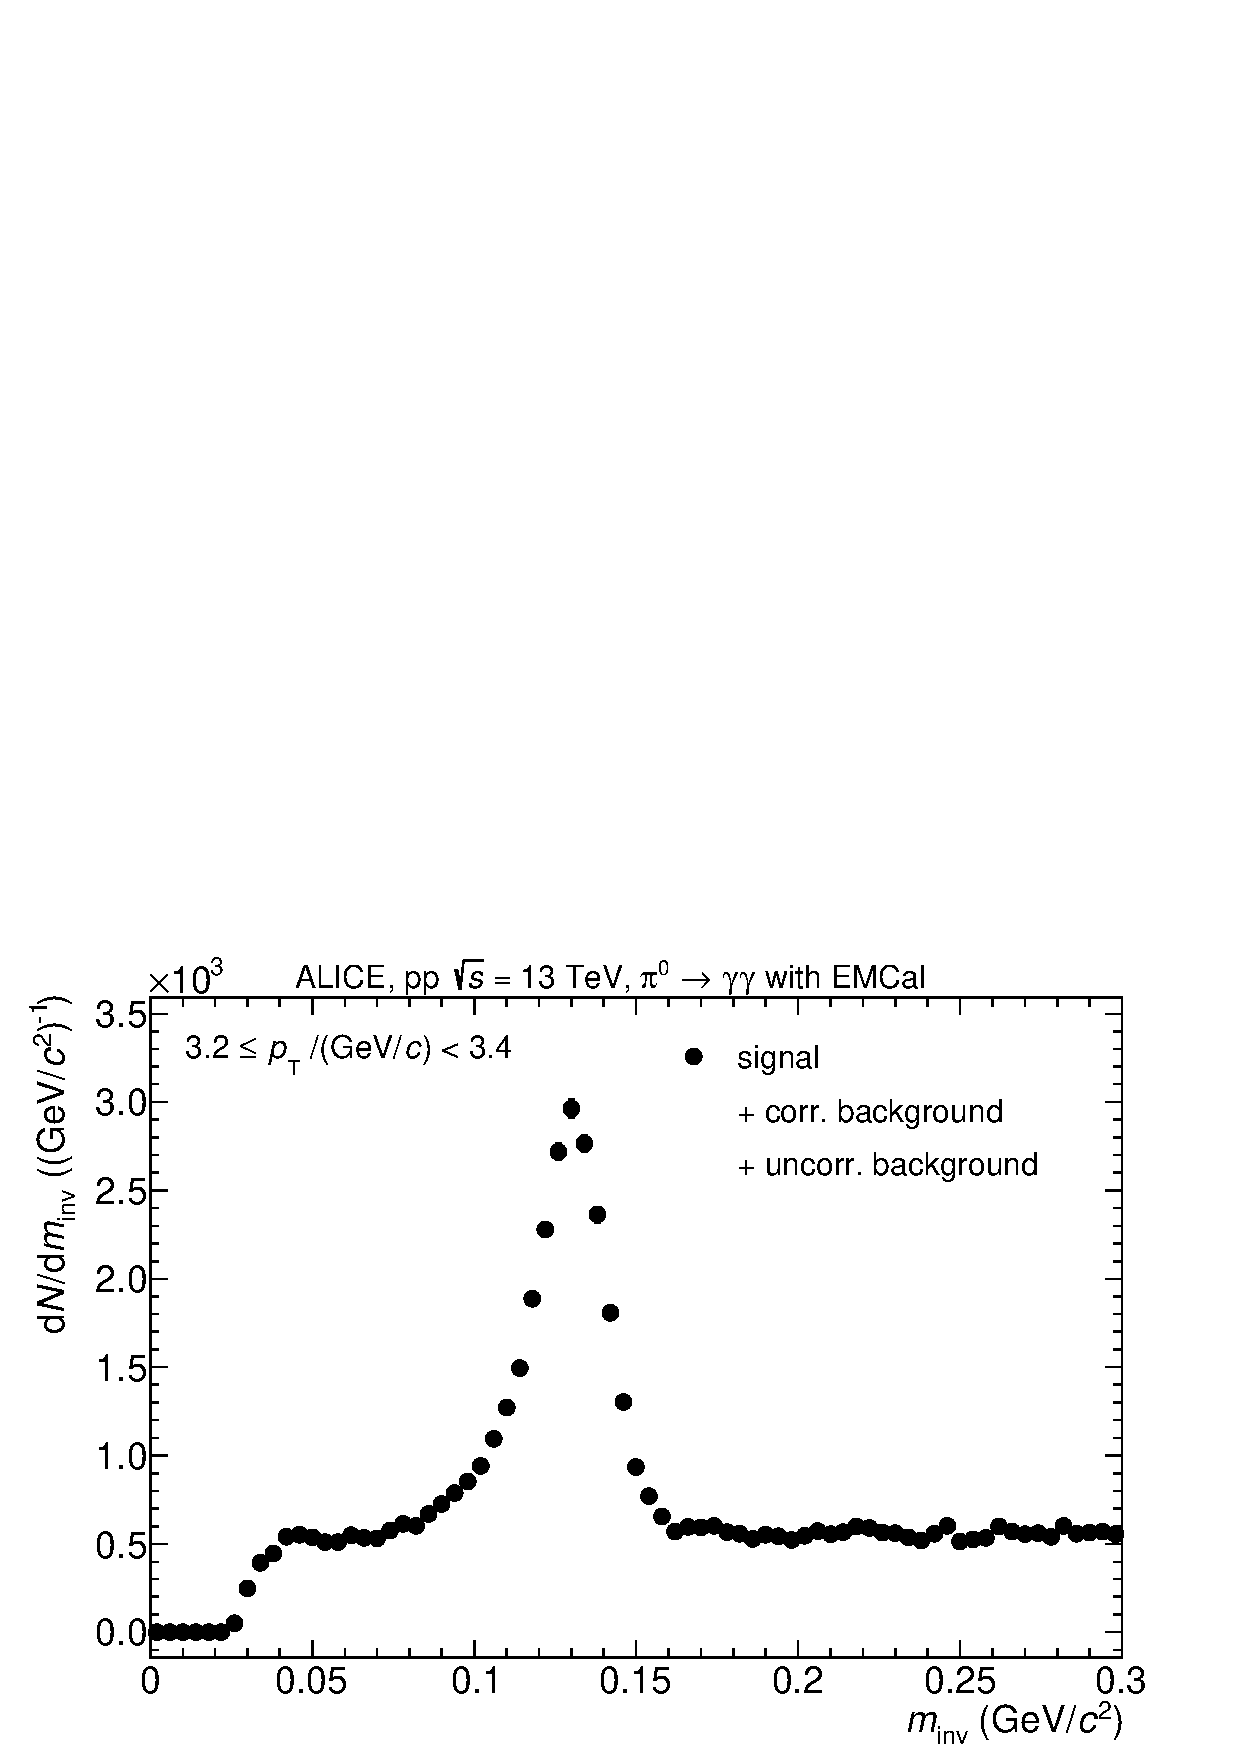
\includegraphics[width=.75\linewidth]{hSignalPlusBkg.pdf}
\caption{Projektion von Abbildung \ref{figInvMassPt_a} im $p_{\text{T}}$-Intervall $(3,2 - 3,4) (\text{GeV/}c)$. Es ist ein deutlicher Peak um $m_{\pi^{0}} \approx 0\,135\text{ GeV/}c^{2}$ zu erkennen, aber auch Untergrund, da das Signal zu höheren Massen gaußförmig abklingen sollte. Bei $m_{\text{inv}} < m_{\pi^{0}}$ kann Signal vorliegen, das aus konvertierten Photonen besteht, weshalb eine Aussage über die Form, beziehungsweise den Untergrund dort schwer möglich ist.}
\label{figSignalPlusBkg}
\end{figure}
\newline
Abbildung \ref{figSignalPlusBkg} zeigt die Anzahl der \textit{Clusterpaare} in Abhängigkeit der invarianten Masse im $p_{\text{T}}$-Intervall von $(3\,2 - 3\,4)(\text{GeV}/c)$.
Die in Abbildung \ref{figInvMassPt_a} beschriebene Anhäufung der Datenpunkten zeigt sich auch hier deutlich und wird im Folgenden als Peak bezeichnet.
Der Peak besteht wie zuvor erwähnt aus Signal.
\newline
Im folgenden Abschnitt wird eine Methode zur Abschätzung des unkorrelierten Untergrunds vorgestellt. 
\subsection{Absch{\"a}tzung des unkorrelierten Untergrunds} \label{s3s3}
\begin{figure}[tp]
\centering
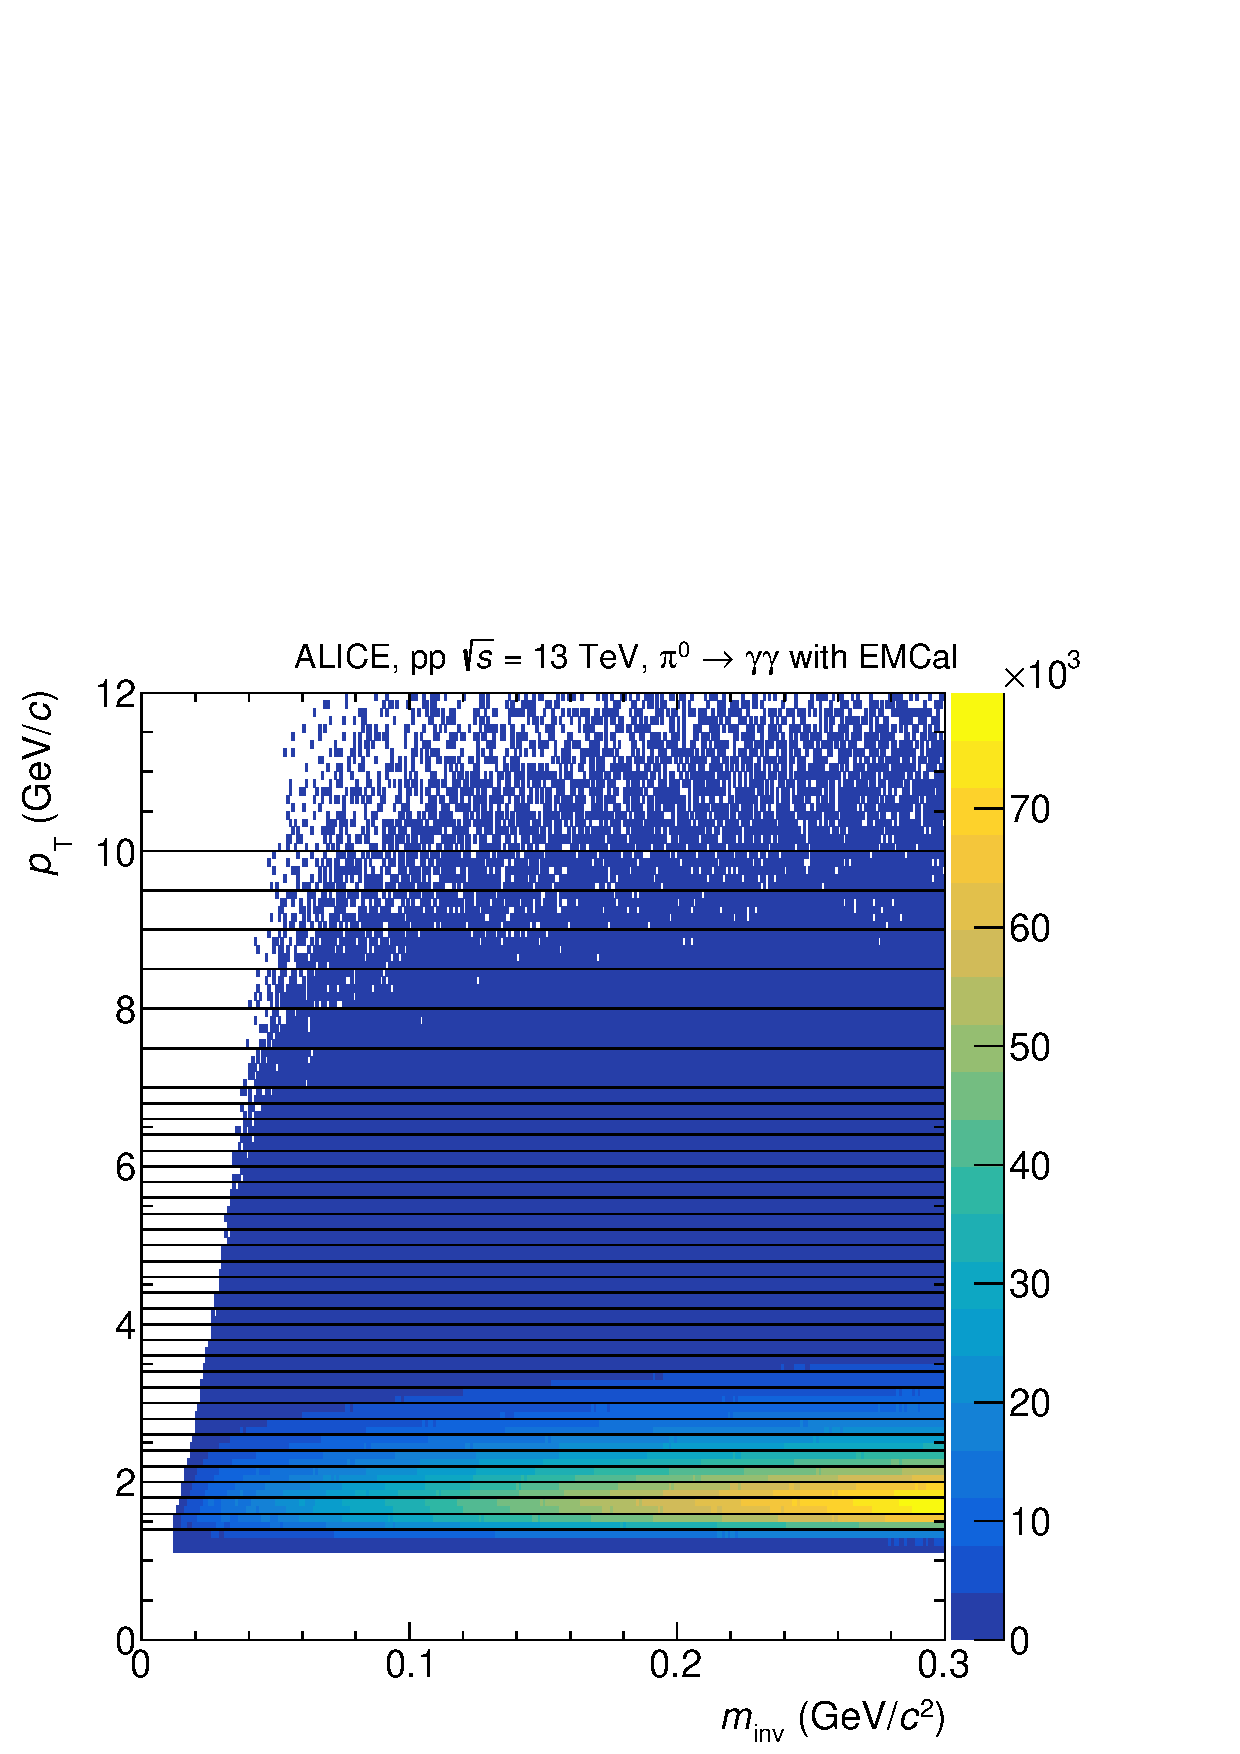
\includegraphics[width=.7\linewidth]{hInvMass_pT_Bkg.pdf}
\caption{$p_\text{T}$ und $m_\text{inv}$ als Funktion von der Anzahl von kombinierten  \textit{Clusterpaaren} aus unterschiedlichen \textit{events}.}
\label{figInvMassPt_b}
\end{figure}
Durch das paarweise Kombinieren aller Photonenkandidaten, wie es in Abschnitt \ref{s3s2} vorgestellt wurde, besteht ein großer Anteil der rekonstruierten Datenpunkte aus unkorreliert Paaren.
Um den unkorrelierten Untergrund abzuschätzen werden Photonenkandidaten aus unterschiedlichen \textit{events} paarweise miteinander kombiniert.
Dadurch wird sicher gestellt, dass zwischen den Photonenkandidaten keine Korrelation besteht.
Diese Methode wird als \textit{mixed event} Methode bezeichnet.
Abbildung \ref{figInvMassPt_b} zeigt eine Verteilung, bei der Photonenkandidaten aus unterschiedlichen \textit{events} miteinander kombiniert wurden.
Eine Häufung der Datenpunkte um eine bestimmte invariante Masse gibt es, wie zu erwarten, nicht.
Durch die Anforderungen an den Öffnungswinkel sind wieder keine Datenpunkte bei kleinen invarianten Massen zu finden.
Die untere Grenze der invarianten Masse, ab welcher Kombinationen möglich sind steigt mit $p_\text{T}$, analog wie zuvor bei Abbildung  \ref{figInvMassPt_a}.
\newline
In der \textit{mixed event} Methode gibt es eine größere Anzahl an Kombinationsmöglichkeiten, als in der \textit{same event} Methode.
Daraus resultiert eine größere Anzahl an Einträgen in der Verteilung der invarianten Masse und des Transversalimpulses, weshalb die Verteilung, die aus der \textit{mixed event} Methode kommt, skaliert werden muss an die Verteilung aus der \textit{same event} Methode.
Die Skalierung erfolgt bei $m_\text{inv} \in \left[0\,19,3\,0\right] (\text{GeV/}c^{2})$, da dort kein Signal erwartet wird.
Es ergibt sich für den Skalierungsfaktor:
\begin{align}
\label{eqBackSkalierung}
\alpha &= \frac{\sum_{i \neq j}\sum_{n}m_{\text{inv}}\left( \gamma^{(n)}_{i},\gamma^{(n)}_{j}\right) }{\sum_{i,j}\sum_{n \neq m}m_{\text{inv}}\left( \gamma^{(n)}_{i},\gamma^{(m)}_{j}\right) }
\end{align}
Die oberen Indize $m$ und $n$ stehen hierbei für ein Event, aus dem ein Photon kommt und die unteren Indize $i$ und $j$ numerieren die Photonen ($\gamma$).
\begin{figure}[tp]
\centering
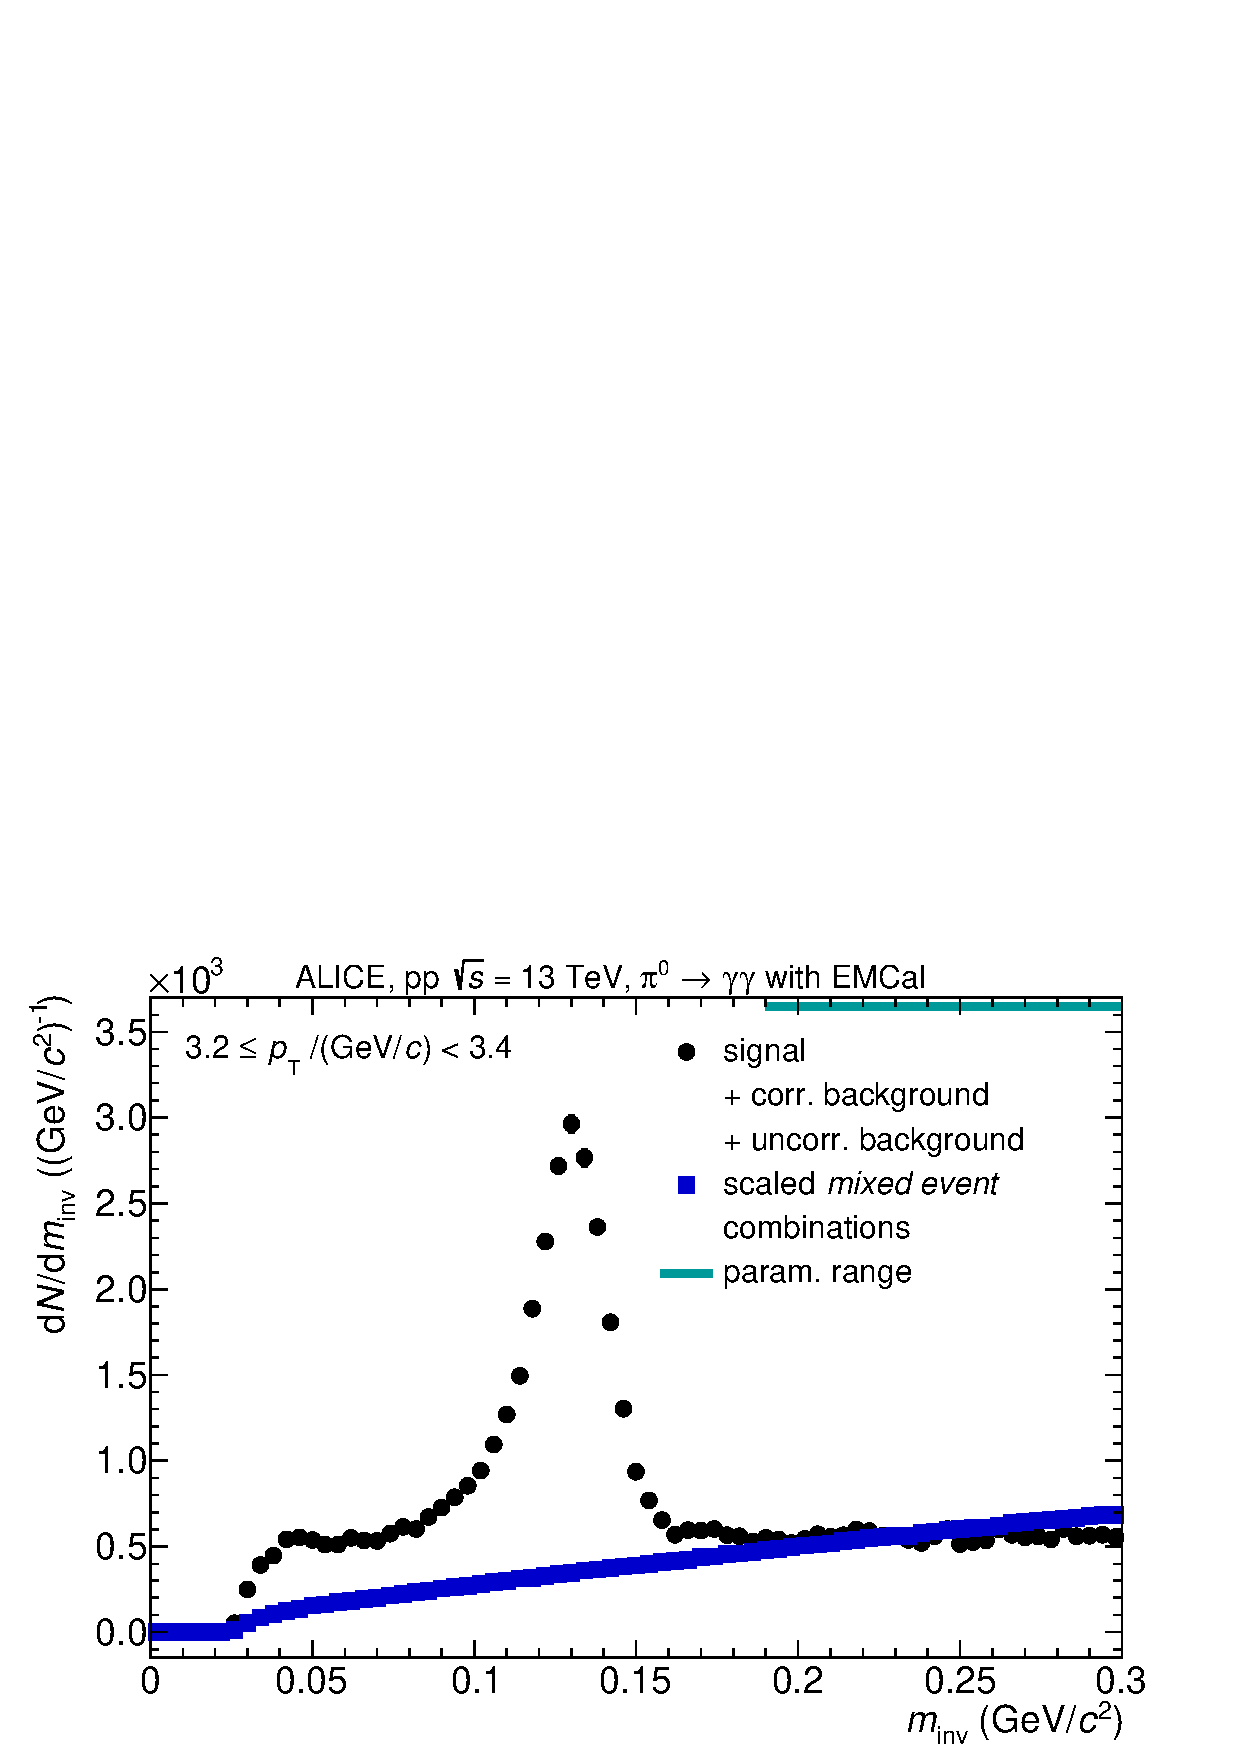
\includegraphics[width=.75\linewidth]{hUncorrBkgNorm.pdf}
\caption{Nach Gleichung \ref{eqBackSkalierung} skalierte {\it mixed event} Kombinationen als Abschätzung des unkorrelierten Untergrunds zusammen aufgetragen mit Signal zuzüglich beiden Untergrundkomponenten wie in Abbildung \ref{figSignalPlusBkg}.}
\label{figUncorrBkgNorm}
\end{figure}
\newline
Abbildung \ref{figUncorrBkgNorm} zeigt die skalierten \textit{mixed event} Kombinationen und das Signal zusammen mit dem korrelierten und dem unkorrelierten Untergrund.
Nachdem der unkorrelierte Untergrund abgeschätzt wird, wird dieser von der Verteilung der invarianten Masse aus der \textit{same event} Methode subtrahiert.
\begin{figure}[tp]
\centering
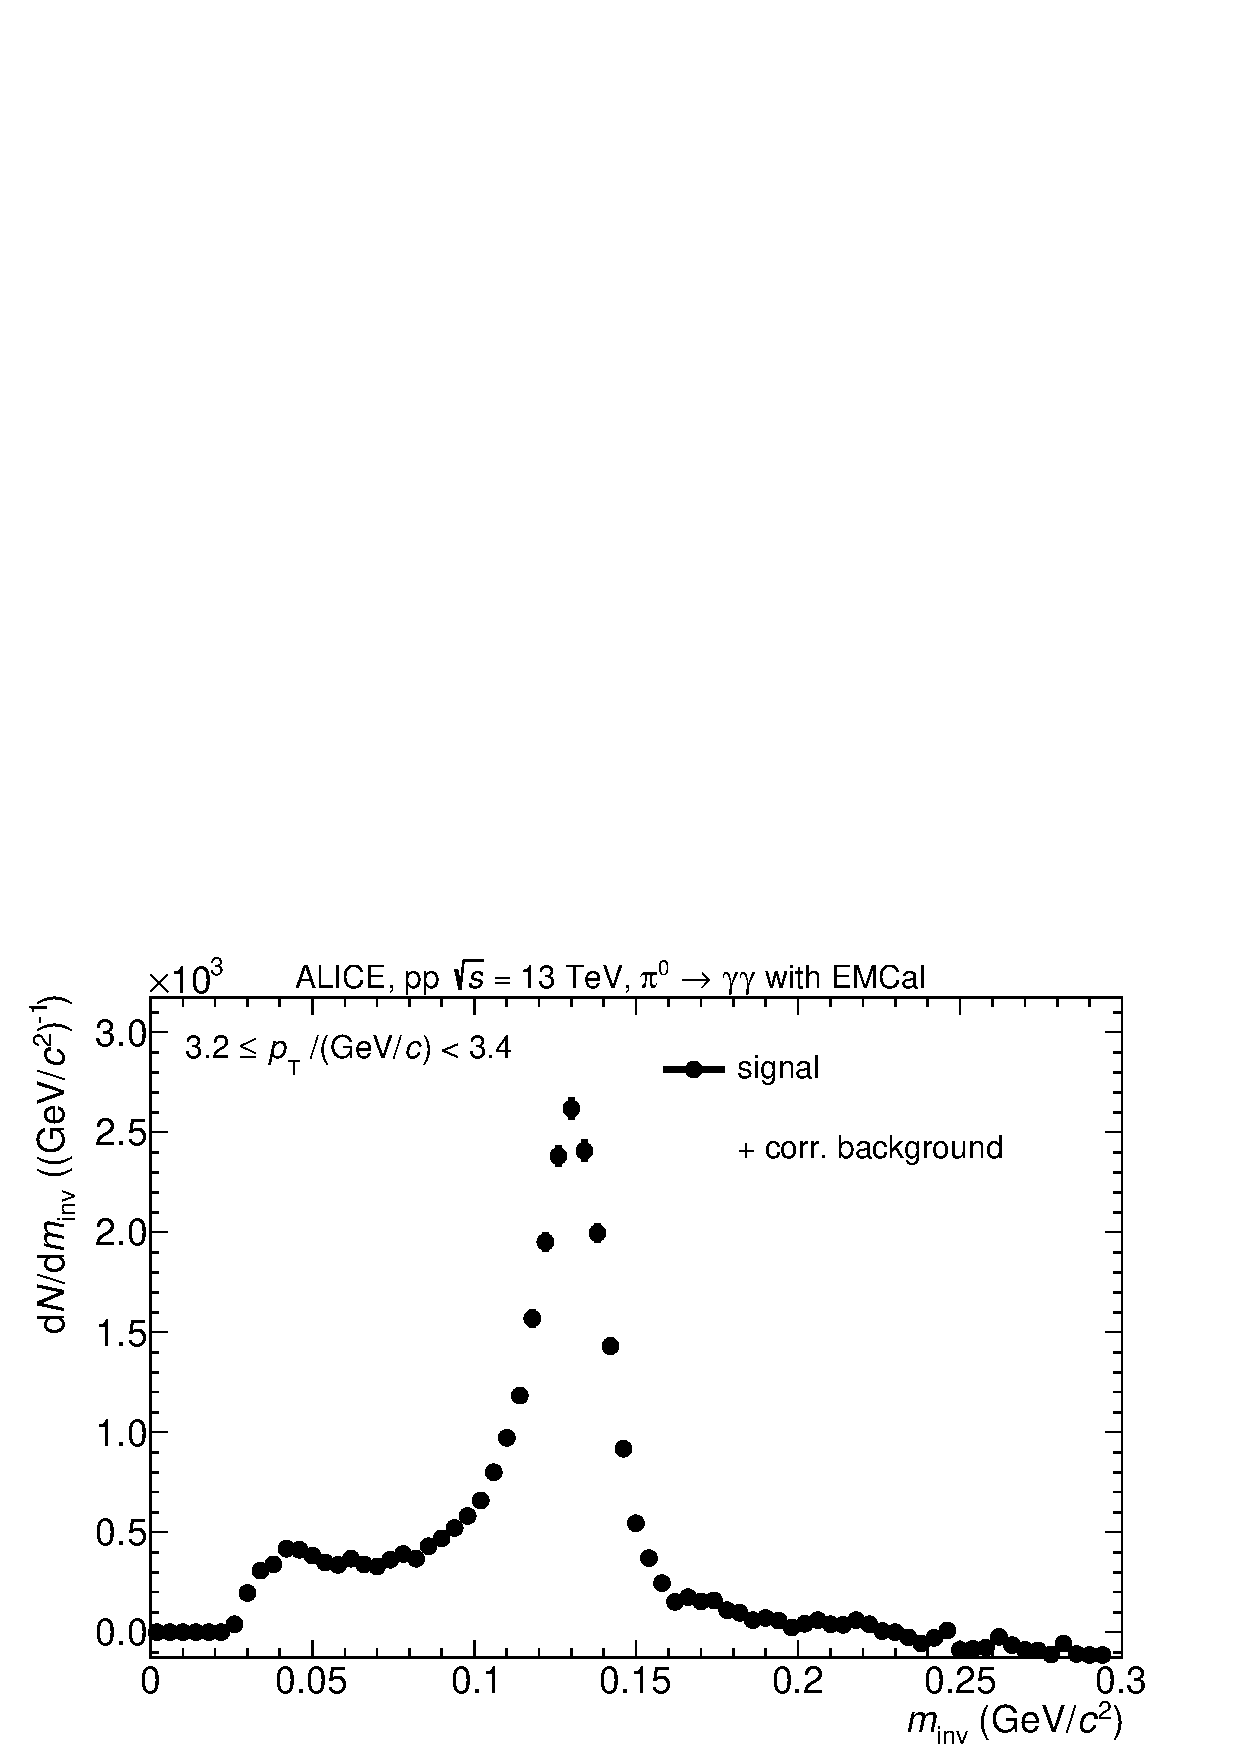
\includegraphics[width=.75\linewidth]{hInvMass_Data.pdf}
\caption{Signal nach Abzug des unkorrelierten Untergrunds.}
\label{figInvMass_Data}
\end{figure}
\newline
Abbildung \ref{figInvMass_Data} zeigt eine Verteilung der invarianten Masse aus der \textit{same event} Methode, nachdem die skalierten Kombinationen aus der \textit{mixed event} Methode, als Abschätzung der unkorrelierten Untergrunds, abgezogen wurden.
Durch die Subtraktion geht jegliche Information verloren, welche Photonenkandidatenpaare welchen Datenpunkt bilden.
Grund dafür ist, dass nicht einzelne Datenpunkte abgezogen werden, sonder lediglich eine gewisse Anzahl an Einträgen.
Deshalb spiegelt die Verteilung eine statistische Auswertung wider, mit statistischen Unsicherheiten.
\newline
Der nächste Schritt in der Analyse neutraler Pionen ist die Bestimmung des korrelierten Untergrunds.
Das Abschätzen mit einer linearen Funktion hat sich als gängigste Methode zur Abschätzung des korrelierten Untergrunds entwickelt und wird im Folgenden als Standardmethode bezeichnet.
In dieser Arbeit wird der korrelierte Untergrund sowie das reine $\pi^{0}$-Signal mit Hilfe von Monte Carlo Templates bestimmt.
Die Ergebnisse der Analyse mit Hilfe von Monte Carlo Templates, sowie mit der Standardmethode werden miteinander vergleichen, um eine Aussage über den möglichen Nutzen von Analysen mit Hilfe von Monte Carlo Templates treffen zu können.
Im folgenden Abschnitt wird zunächst die Standardmethode kurz erläutert.
\subsection{Peak Extraktion mit Hilfe von Parametrisierungen von Funktionen} \label{s3s4}
Da es sich bei dem Signal ohne Konversionsanteil um eine statistische Größe handelt, wird eine gaußförmig Funktion benutzt, um dieses zu beschreiben.
\newline
Der Konversionsanteil des Signals wird als \textit{Tail} Komponente bezeichent.
Diese Komponente wird durch eine exponentielle Funktion und einer gaußförmige Funktion beschrieben.
Sie dient der Abschätzung des Anteils des Signals, dem Konversionselektronen oder Konversionspositronen zu Grunde liegen.
Für die Abschätzung des korrelierten Untergrunds wird eine lineare Funktion angenommen.
Die drei Funktionen werden kombiniert an die Verteilung der invarianten Masse angepasst.
\begin{figure}[tp]
\centering
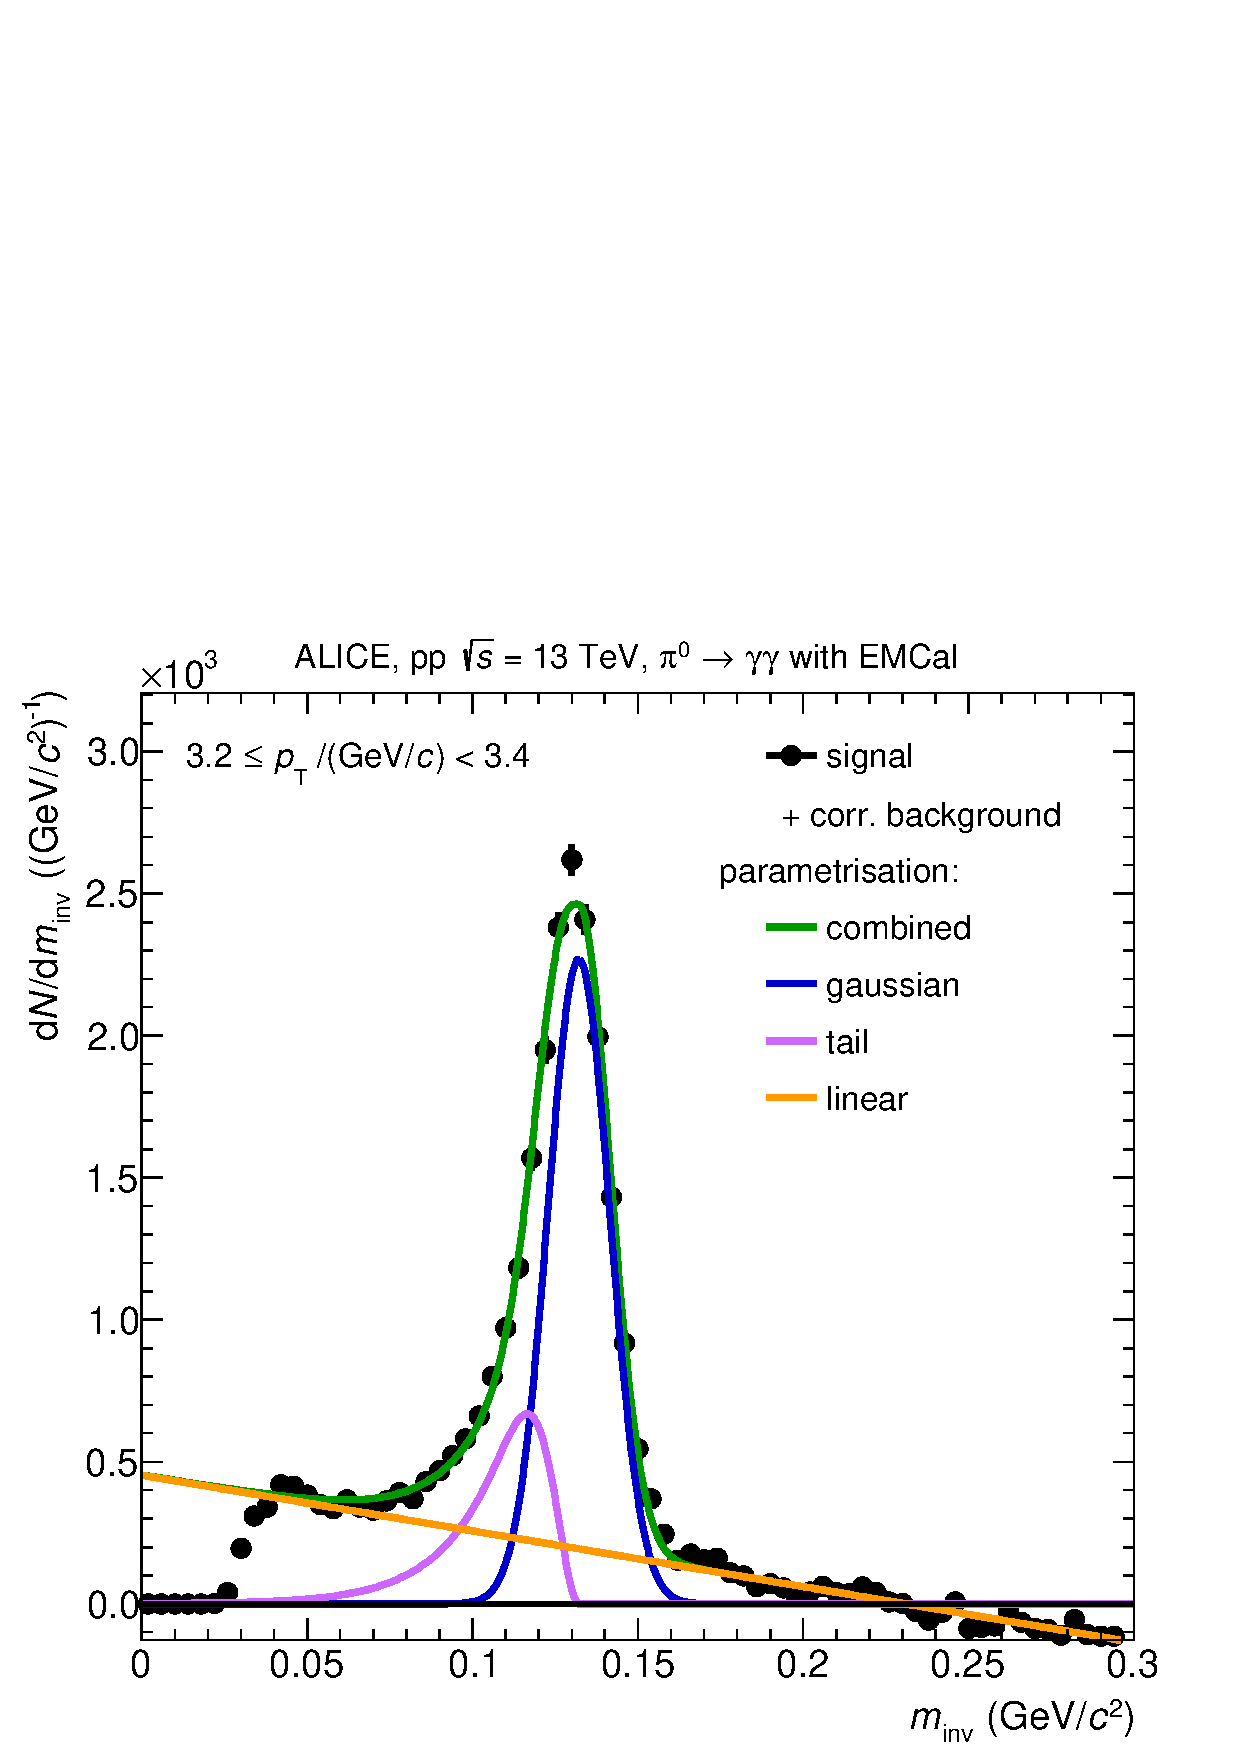
\includegraphics[width=.75\linewidth]{StandardParam.pdf}
\caption{Signal mit korreliertem Untergrund sowie den Funktionen zur Beschreibung des Signals mit korreliertem Untergrund.}
\label{figStandardParam}
\end{figure}
\newline
Abbildung \ref{figStandardParam} zeigt die Verteilung der invarianten Masse, bestehend aus Signal und korreliertem Untergrund, sowie das Ergebnis der an die Daten angepassten Funktion.
Die grüne Funktion entspricht der Summe der drei einzelnen Komponenten, wobei die Gauß-Funktion in blau, die \textit{Tail}-Funktion in pink und die lineare Funktion in orange dargestellt sind.
Dabei wird deutlich, dass durch die Abschätzung des korrelierten Untergrunds über die lineare Funktion bei $m_\text{inv} < 0\,06\text{ GeV}/c^{2}$ kein Signal erwartet wird.
Für $m_\text{inv} < 0\,02\text{ GeV}/c^{2}$ gibt es keine Einträge in der Verteilung aufgrund des minimalen Öffnungswinkels.
Dieses Verhalten wird nicht von der Abschätzung des korrelierten Untergrunds berücksichtigt.
\newline
Um die Anzahl der produzierten $\pi^{0}$ mit der Standardmethode zu bestimmen, wird die Anzahl der Einträge, die unter der lineare Parametrisierung liegen, von der Summe der Einträge der Daten abgezogen.
Anschließend werden die übrigen Daten, also das Signal, über einen festen Bereich um den Erwartungswert der Gauß-Funktion integriert.
Für eine detaillierte Beschreibung der Standardmethode sei an dieser Stelle auf \cite{thesis:Adrian} verwiesen.
\newline
Im folgenden Abschnitt wird die Abschätzung des korrelierten Untergrunds mit Hilfe von Templates beschrieben.

\subsubsection{Absch{\"a}tzung des korrelierten Untergrunds} \label{s3s4s1}

\subsection{Peak Extraktion mit Hilfe von Parametrisierungen von Templates} \label{s3s5}

\subsubsection{Template des Signals} \label{s3s5s1}

\subsubsection{Template des korrelierten Untergrunds} \label{s3s5s2}

\subsubsection{Parametriesierungsmethode} \label{s3s5s3}

\subsubsection{Abzug des korrelierten Untergrunds und Integration des Signals} \label{s3s5s4}
\newpage
\section{Korrigierter Yield} \label{s4}

\subsection{Korrekturen} \label{s4s1}

\subsection{Systematische Unsicherheit} \label{s4s2}

\section{Zusammenfassung und Ausblick} \label{s5}

\newpage
\bibliography{bib_bath_mahe} 
\bibliographystyle{alpha}

\end{document}
